\documentclass[11pt,oneside,a4paper]{article}
\usepackage{graphicx}
\usepackage{hyperref}
\usepackage{float}
\usepackage{amsmath}

\title{Strace in XV6}
\author{Xiang Mei \\ \href{mailto:xm2146@nyu.edu}{xm2146@nyu.edu} }

\begin{document}
\maketitle
\section{Introduction}

\begin{figure}[H]
    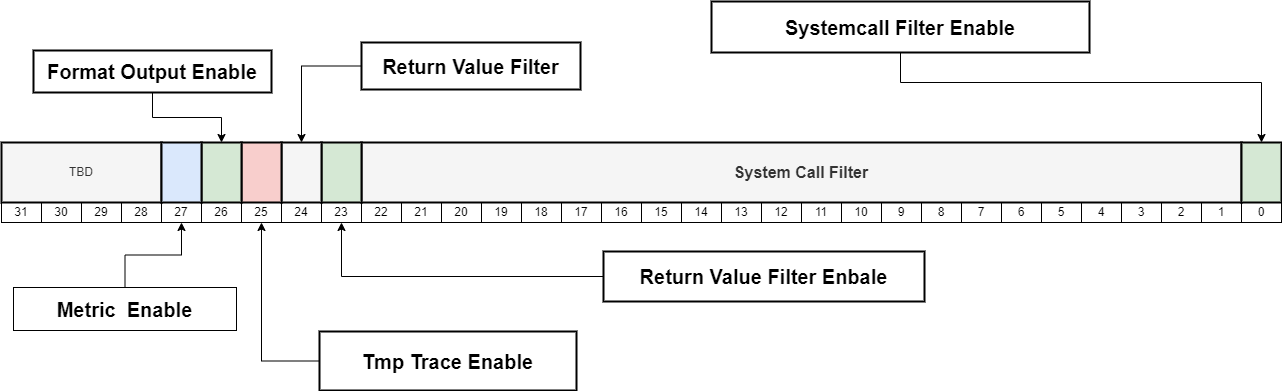
\includegraphics[width=4.75in]{pstrace.png}
    \centering
    \caption{My Strace}
\end{figure}

Strace is a very useful tool on Linux. It's widely used to perform troubleshooting.
But we don't have preinstalled strace on XV6. I'll implement a simple strace on XV6.

It sounds like reinventing a wheel. But for my experience in this course, Intro to OS,
I think writing a simple version of the "wheel" could help me to understand the
complexity of the "wheel" and help me think like an engineer. We need to consider
lots of questions during the implementation, such as "why should the wheel be 
round?". Anyway, I learned a lot and used some skills I learn from the previous assignment.

The first section is the introduction of the report and I'll document my design in the
second section. The real task-related parts start from section 3.

\paragraph*{Information for TA team}

My strace could satisfies all the requirments in the write-up, including
"strace on", "strace off", "strace run command", "strace dump", "Trace child process", 
"Option: -e system-call-name", "Option: -s", "Option: -f", 
"Option runs only once", "Write output of strace to file", and "Application of strace".

Also, my strace satisfies all the extra credits, including 
"Extra credits: Formatting more readable output", 
"Extra credits: Combine options", and 
"Extra credits: Implement -c options".

All explanations and screenshots are in Section 4 Design;
The README file of this assignment is at /README.MD;
"A text that state your partner or working alone" is at /FYI.MD;
and you can find "Application of strace" content in section 5.

\section{Get familiar with Linux strace}
In order to get familiar with the real strace, I use it to trace the sleep command.
After reading the help page of strace, I use the "-C" flag to show the list of called
syscalls, total number of calls, and time of running strace on command.

\begin{figure}[H]
    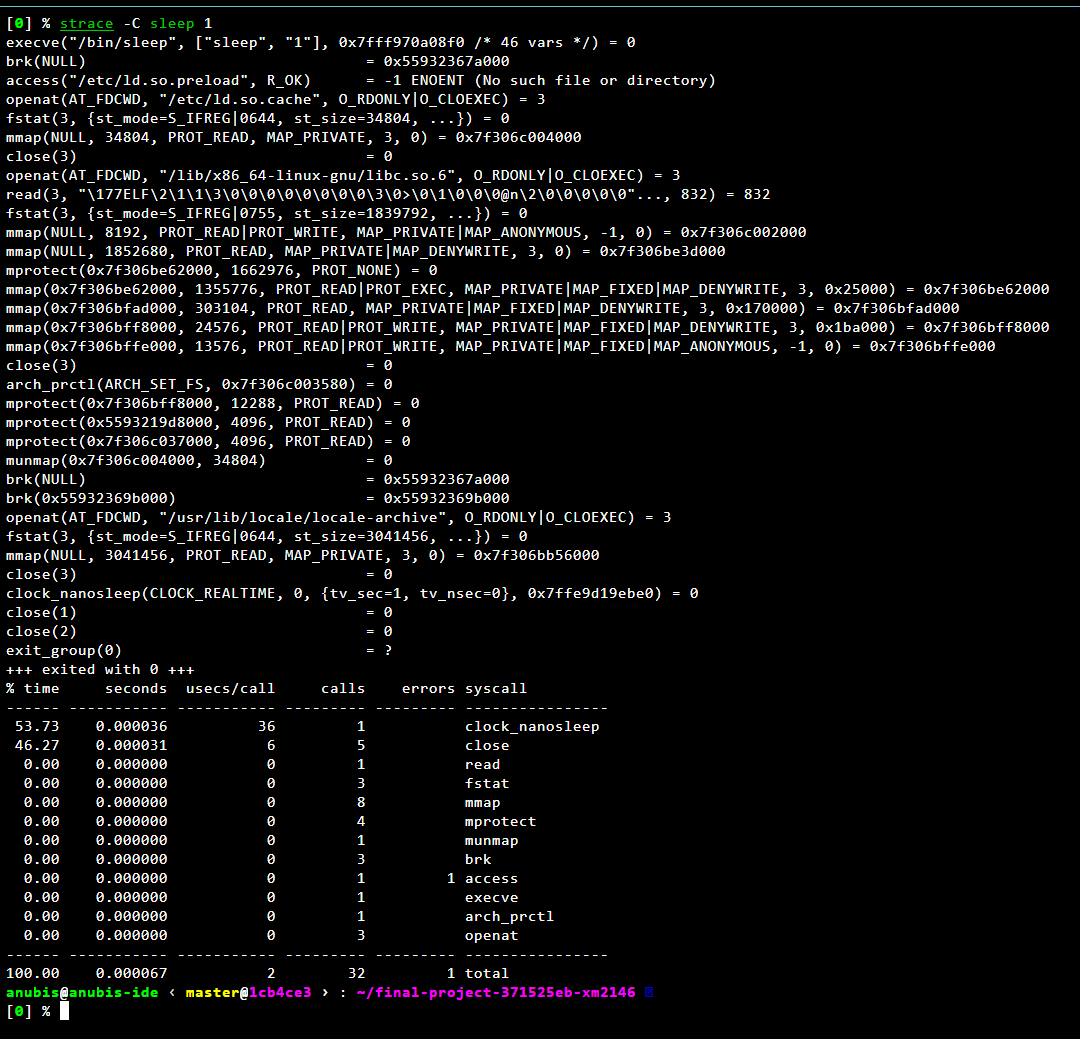
\includegraphics[width=4.75in]{1-3.png}
    \centering
    \caption{Task 1-1}
\end{figure}

For tasks 1-2, I choose "mmap, read, execve, mprotect" as the targets to explain. We can
see the procedure clearly in the above figure. The "execve" call is called once and 
that's the first syscall we called. The "sleep" is an executable file in our system
and the execve syscall could run it. It's worthy to mention the executed binary would 
use the caller's memory space and proc struct. By the way, the execve syscall has three
3 parameters, the first one is the path of the executable binary. And the second one
would store the arguments while the third one would store the environment parameters.


The mmap syscall is used to allocate a large chunk of memory. In our command, 
it's used to allocate memory to store the shared libraries, the linker, and other 
needed files. As we can see in the above figure, mmap is usually called after openat.
The first parameter of mmap syscall is the address of the allocated chunk. You can 
set it NULL to represent an arbitrary address and we can also set it to a non-NULL value
to get a chunk strat from that address. This is used to allocate more space based 
on a known chunk. The second parameter is the length we want to allocate while the third
argument is the permission of the chunk, such as readable, writeable, and executable.

And the mprotect is used to change the permission of memory. The mprotect can't 
allocate new memory. It could only change the permission of the memory chunks. 
In our command, it's used to make mmaped memory not writeable. For example, we 
allocate a chunk for the shared libraries and the memory must be writeable because
we need to copy the bytecodes to the memory. But you know it's dangerous to make writeable
memory executable. So we need mprotect to make it un-writeable after copying.

The syscall read is kind of straightforward. It reads the content from the first parameter's
corresponding file and stores the content in the second parameter's correct memory while the third
parameter is the max length of content the read syscall could read. It's used once to 
read the header of our glibc.

So far, we go through the usage and the shown information of strace on Linux.
Strace is a useful tool and I have been using it for a long time but I still 
find something new by reading its help page. And we are going to implement 
out strace.

\section{What features do we need}

In this assignment, we gonna implement a simple strace. I'll go through and features 
needed. 

For my implementation, the command should be like:

\begin{figure}[H]
    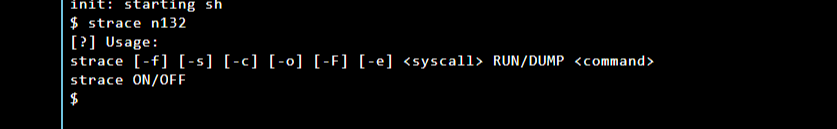
\includegraphics[width=4.75in]{1-4.png}
    \centering
    \caption{Usage}
\end{figure}

We have 4 sub-commands("RUN", "DUMP", "ON", and "OFF"), 3 filter options("-e","-s",and "-f"),
and 3 output control options("-F","-c", and "-o").

I'll introduce these options and sub-commands in a later section. And there are a short 
version introduction: The sub-command "RUN" could strace the following command and 
trace the syscall until the following command exits and the "DUMP" would dump the 
syscall records in the kernel. Also, we can use "strace on" to ask the kernel to keep
recording syscalls while the "strace off" could get the kernel back to the normal mode.

If we add "-e" options, the strace would only record and print specific syscalls. 
Besides, the "-s/f" flag would force the strace to only record and print successfully/failed
syscalls. 

Moreover, we have output control options. The "-F" flag would print more readable 
output and the "-c" would print a table of syscall metrics. As for "-o", it can set 
an output file and the strace's output would be stored in that file.

\section{Design}

This section will tell you the reasons for my design. 
This time, not like the "uniq" assignment, our implementation is different 
from the real sample because we don't have pthread syscall in xv6. Also, the 
strace is a big project I don't have much time to read its code. So during the 
implementation, I try to solve the problem myself and look up the materials when 
I don't have an elegant solution.

\paragraph*{ON/OFF}

\begin{quotation}
    "When typing 'strace on' in the terminal, the mode of strace is on, and therefore the next type in
command will be traced. The system call list will be printed on the screen in format PID (process id),
command name, system call name, return value."
\end{quotation}
The "ON/OFF" implementation is easy and straightforward. In the requirements, we need
to print the PID, name, and syscall of processes. Obviously, we can't do this task
in userspace. I create a global variable in kernel space to present the current 
strace\_mode.
\begin{figure}[H]
    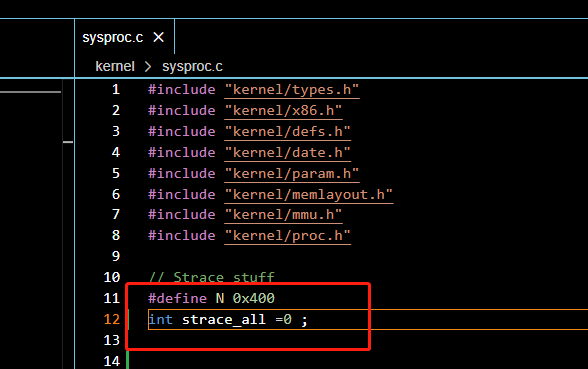
\includegraphics[width=4.75in]{1-5.png}
    \centering
    \caption{Strace All}
\end{figure}
Like what shows in the above figure, I set a global variable in "sysproc.c" because I'll
later implement a syscall as a bridge to transfer commands from user space to the kernel.

\begin{figure}[H]
    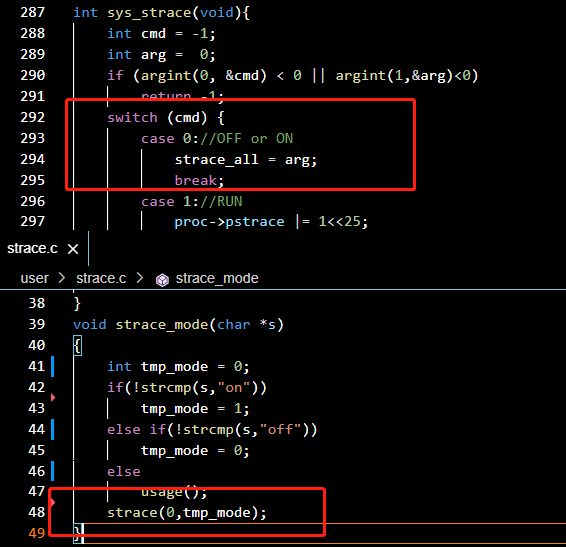
\includegraphics[width=4.75in]{1-6.png}
    \centering
    \caption{Strace Syscall}
\end{figure}
As you can see in the above figure, I parse the parameters from the command line and 
use strace syscall to modify the kernel variable. Basically, we can use the code above
to control the strace mode from userspace. Nevertheless, how do we monitor the 
syscalls?

At very first, a simple plan came up in my mind: I can insert a piece of code into every
syscall so that I can print the result and parameters when running the syscall. 
And I use a global variable "strace\_all" to tell the system if we should print the
strace info while calling syscalls. But quickly I found there are some serious 
issues with this solution. We have 21 syscalls and if we need to write different 
strace\_handle for every syscall and it's not convenient because we may need to 
modify 21 places for every single change. My experience told me it's horrible. 
We must implement something more elegant.

The advantage of the previous plan is that we can print the arguments of syscalls.
If we need to print the content of the syscall we have to do that because the 
syscalls would parse the parameters in these syscall handlers. I asked in slack 
and found we don't need to print the details about the syscall so that we can
move the strace code to the syscall\_interupt handle or the wrapper function.

\begin{figure}[H]
    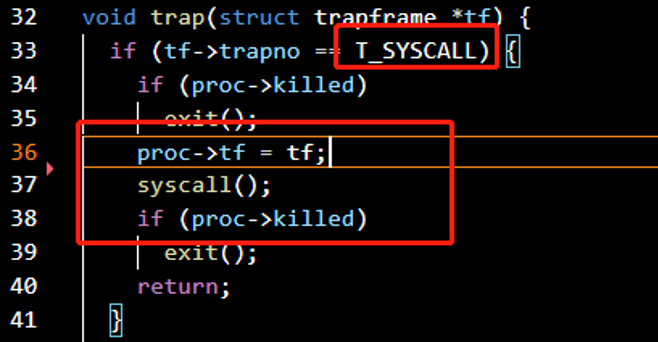
\includegraphics[width=4.75in]{1-1.png}
    \centering
    \caption{Syscall Handler in Trap Fcuntion}
\end{figure}

As we talked about in this trap section, the syscall in userspace would use create an
interrupt to inform the kernel. And the interrupt is handled by the function alltraps 
in "trapasm.S" it would store the current context in the trap frame and call the function 
trap which is shown in the above figure. And we can see the trap would check the 
process's state and call the function syscall. This function is in file syscall.c.

\begin{figure}[H]
    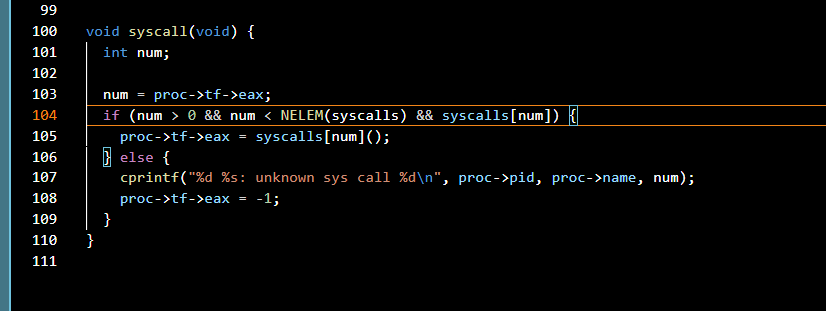
\includegraphics[width=4.75in]{1-2.png}
    \centering
    \caption{Syscall Wrapper}
\end{figure}

In this function, we would parse the EAX which represents the syscall index, and 
store the return value in the EAX. So I think this function is a good candidate
to insert our strace code. 

\begin{figure}[H]
    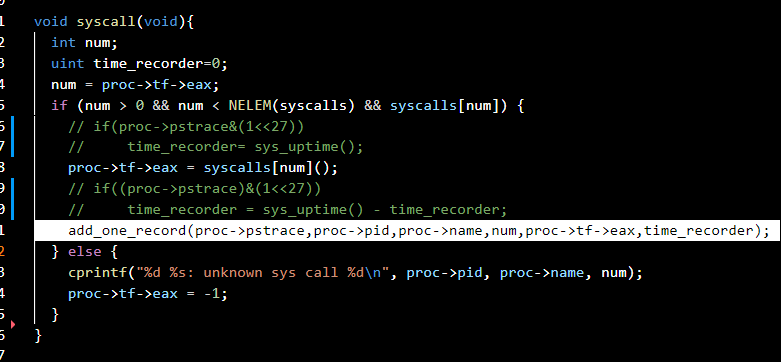
\includegraphics[width=4.75in]{1-7.png}
    \centering
    \caption{Monitor}
\end{figure}

I insert the monitor after the syscall because we need the return value of the syscall
but we may lose the "exit" syscall because the process would stop in the "exit" syscall. 
So I add the same function before the process really exits which is shown in figure 8.

\begin{figure}[H]
    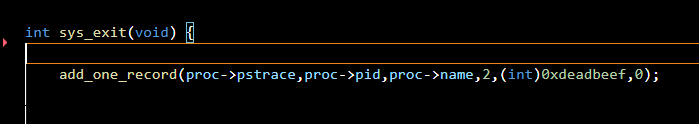
\includegraphics[width=4.75in]{1-8.png}
    \centering
    \caption{Strace Handler in sys\_exit}
\end{figure}

The usage of this sub-command is simple. You can just use "strace on" to turn on
strace and "strace off" to turn off strace.

\begin{figure}[H]
    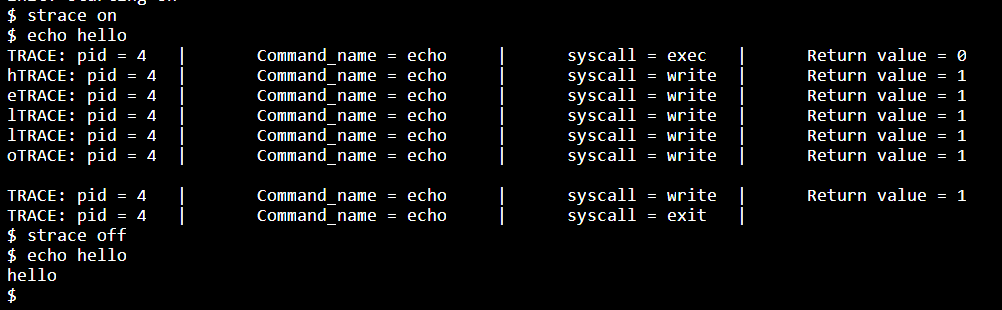
\includegraphics[width=4.75in]{1-13.png}
    \centering
    \caption{Strace On and OFF}
\end{figure}

There is nothing more about these 
two sub-commands but there is a little problem with the global variable. In order for 
avoiding race conditions, we need to implement a lock mechanism for this variable. However,
this is not the requirement for this assignment and there is only one member on my team. 
I decide to implement that only if I have time left.




\paragraph*{DUMP}
\begin{quotation}
"Implement a kernel memory that will save N number of latest events. This N number can be
configurable by using define in XV6. In order words, it can be hard to code but the way to implement
is to use define to declare a variable called N with a certain value. When 'strace dump' command is
called, print all events that are saved in kernel memory."
\end{quotation}
In previous figures, you may notice that I implemented a function to log the syscall.
so why do I implement a such complex function "add\_one\_record".

For implementing the "DUMP" feature, we need to allocate a space in the kernel to store
the latest N system calls. These data have to be stored in the kernel space as a global 
variable because xv6 is a multi-process system. And we need a special circle buffer to
store the latest N records.

\begin{figure}[H]
    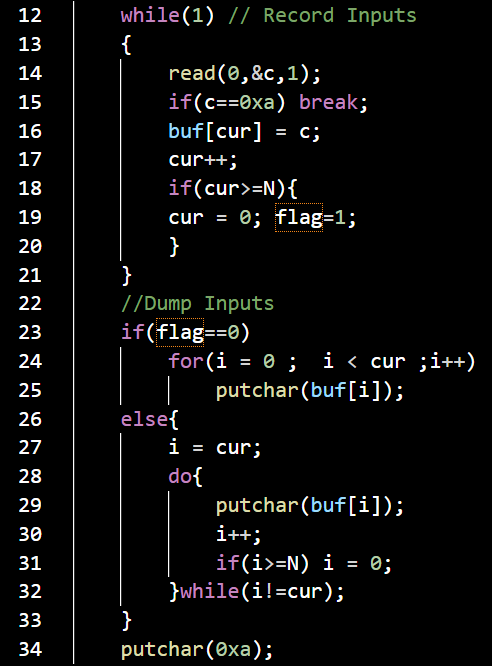
\includegraphics[width=4.75in]{1-9.png}
    \centering
    \caption{Circle Buffer}
\end{figure}

The circle buffer for DUMP operation is easier than the general circle buffer. First, I 
implemented a C code version for testing. As you can see in the above figure, 
We read the input to the circle buffer and dump the content when we get an "enter".
The read-part is simple and the "flag" variable is important. It decides how many
and where to dump. The trick in the code is simple and makes sure we would print the
last N records which are verified by my fuzzer. That's another reason why I write it 
in C. Also, I attach my fuzz code:

\begin{figure}[H]
    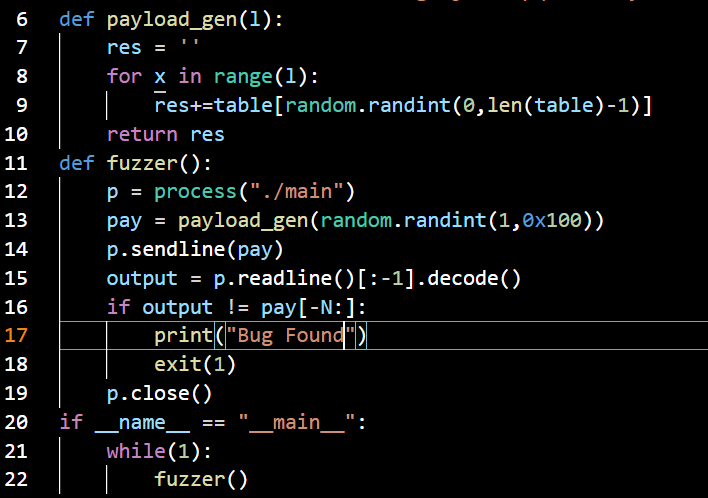
\includegraphics[width=4.75in]{1-10.png}
    \centering
    \caption{Circle Buffer Fuzzer}
\end{figure}

After another test, I implement a similar circle buffer in the kernel to store and 
dump the syscalls. In function "add\_one\_record", I record the syscall's information in 
the correct node and move the pointer like what I did in my previous demo. 

\begin{figure}[H]
    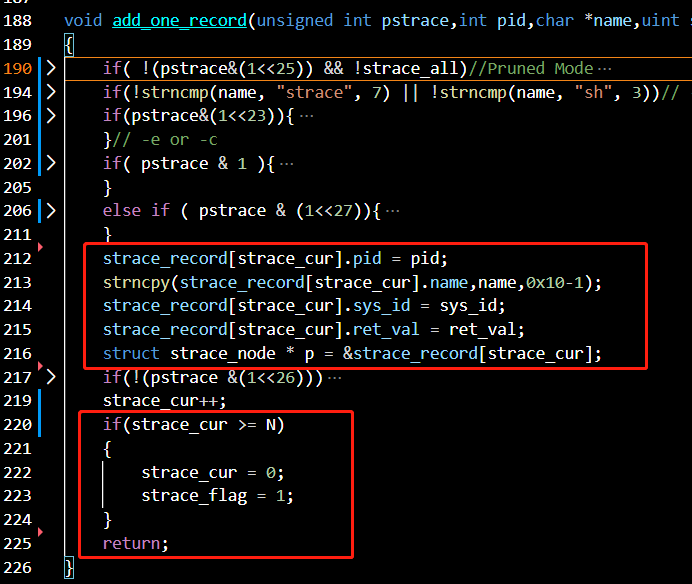
\includegraphics[width=4.75in]{1-11.png}
    \centering
    \caption{Circle Buffer Fuzzer}
\end{figure}

That's the key function of all my designs I'll mention this function later to introduce 
other features. This function is only called in function syscall and sys\_exit so that
if we want to modify, delete, or add a feature to strace, we can just modify the code 
in this function. Another advantage is that we can naturally combine kinds of options.

\begin{figure}[H]
    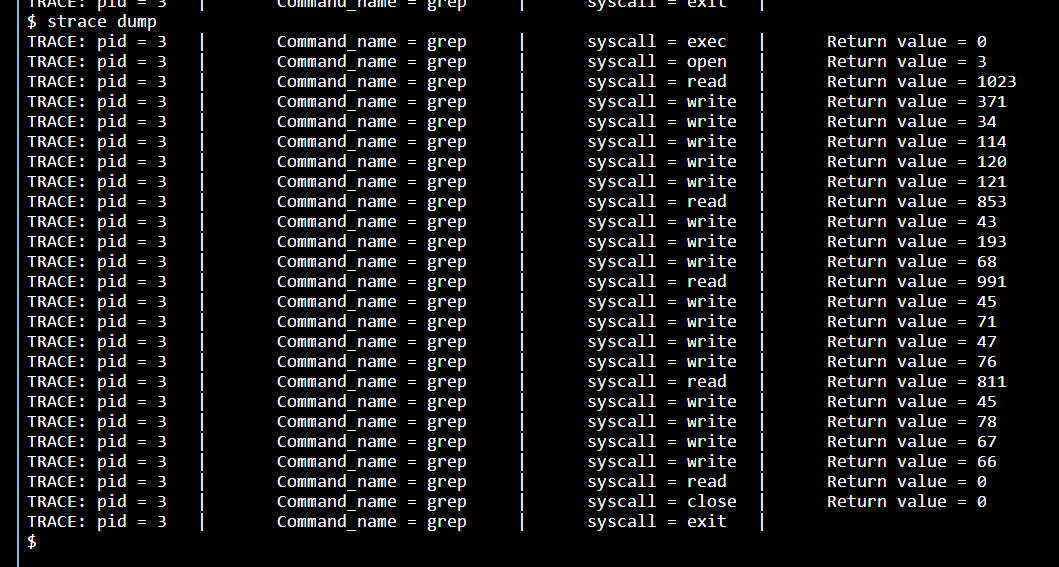
\includegraphics[width=4.75in]{1-12.png}
    \centering
    \caption{DUMP after Traing "grep the readme.md"}
\end{figure}

I did several tests on DUMP and it works well. I attach a simple sample above because 
the output of a complex test case would be big and hard to recognize. 
You can also test it with any commands you like and please check the README.md file 
attached to the assignment submission.

\paragraph*{RUN}

\begin{quotation}
    "Instead of turning on and off strace, we create 'strace run' to directly point tracing to the current
process that executes the command. For example: when typing 'strace run echo hello' in the
terminal, we get the output tracing of echo hello."
\end{quotation}

For sub-command "RUN", we gonna run a command and strace the syscall of the command.
So we can parse the parameter and use the "fork" or "exec" syscall to run the command.

I used the "exec" syscall for my strace and there is a disadvantage compared with 
the fork version. I know the fork version from my professor: 
we can use "fork" to create a child process and let the parent process wait for the 
metadata of outputs from the kernel. So all the output parts would be handled in user 
space which is much more secure and beautiful. However, I have almost finished my implementation
and there is not much time for this huge modification. Therefore, I'll keep my "exec"
version and for my implementation, I think they are similar in complexity.


\begin{figure}[H]
    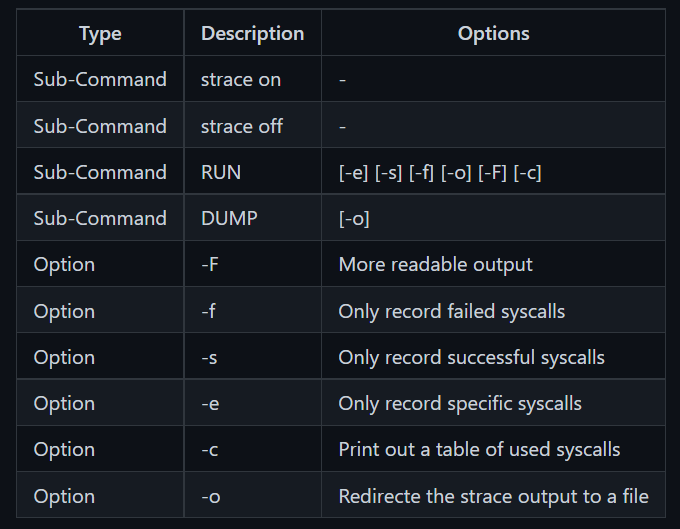
\includegraphics[width=4.75in]{1-39.png}
    \centering
    \caption{Supported Opetions}
\end{figure}

The "RUN" sub-command is the most complex part of my strace, I'll introduce some 
basic ideas about this sub-command in this parameter and explain the rest parts with
the supported options. So how can we strace one command once?

If we "RUN" a command, we are going to use "fork" to create a new process or use 
"exec" to run an executable file by using current memory space. We must have a way to 
pass the information that the new process should be traced. In order to implement this,
I add a new element in the "proc" struct in proc.

\begin{figure}[H]
    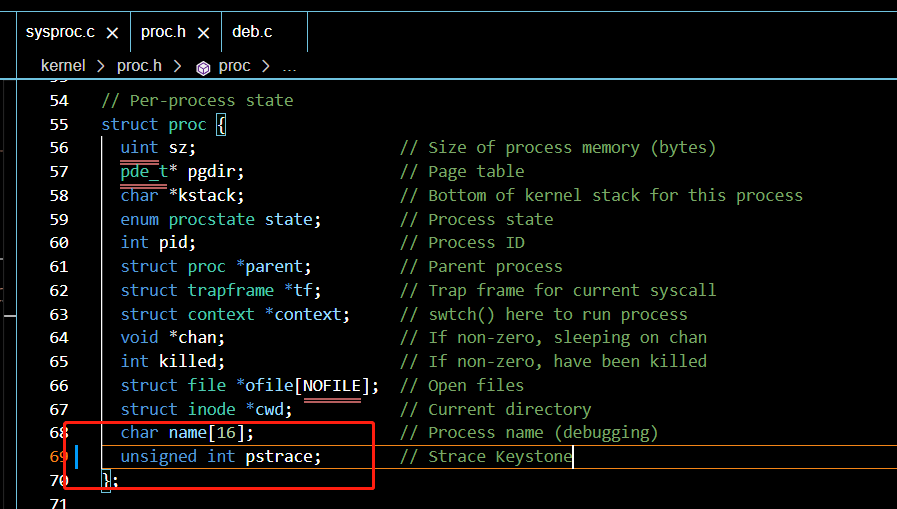
\includegraphics[width=4.75in]{1-15.png}
    \centering
    \caption{Strace a Process}
\end{figure}

As you can see in the above figure, I add an unsigned integer to the proc struct.
I don't want to waste unnecessary space in the kernel space.
so I would use this 4 bytes variable to store all the strace information such as 
output filter information and output format information. I'll explain the struct of
this variable in the option-related paragraph.

\begin{figure}[H]
    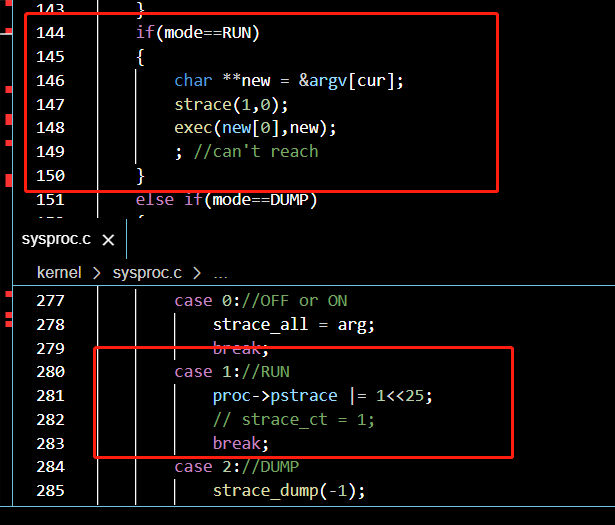
\includegraphics[width=4.00in]{1-16.png}
    \centering
    \caption{RUN Sub-command in User Space}
\end{figure}

The above figure is my userspace interface and corresponding system call implementation.
As you can see I use the 26th bit of the "pstrace" to sign if the kernel should strace
the process. Another advantage of having a variable in the "proc" struc is that we can 
easily follow the subprocess by modifying the "fork" function in "proc.c".

\begin{figure}[H]
    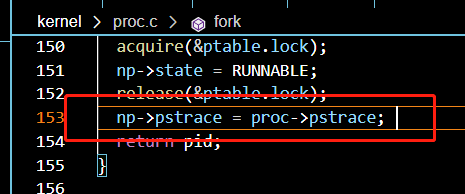
\includegraphics[width=4.00in]{1-17.png}
    \centering
    \caption{Trace the Child Processes}
\end{figure}

Now we can use strace to run strace any process! There is a simple demo of "RUN" 
sub-command.

\begin{figure}[H]
    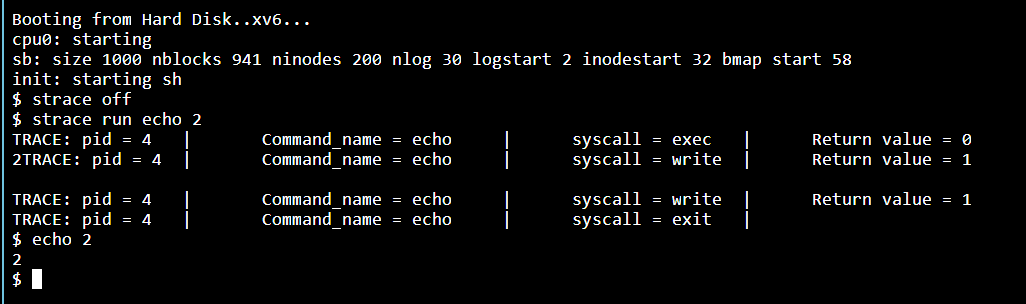
\includegraphics[width=4.75in]{1-18.png}
    \centering
    \caption{Strace RUN}
\end{figure}

\paragraph*{Opetions}

\begin{quotation}
    My strace supports kinds of output filter and format options which could help to 
eliminate the uninterested syscalls. 
\end{quotation}

\begin{figure}[H]
    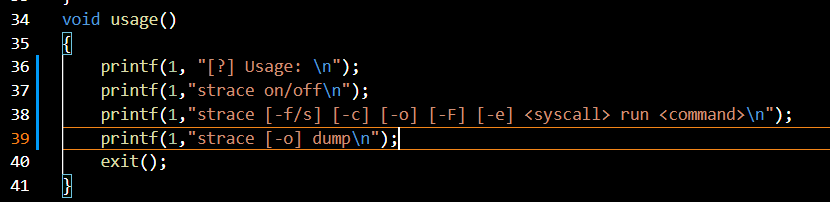
\includegraphics[width=4.75in]{1-19.png}
    \centering
    \caption{Supported Opetions}
\end{figure}

I would parse the parameters in the user space and use the strace syscall to 
pass the operations to the kernel mode. 
As we talked about in the previous paragraph, the atomic unit of strace is the process so 
we need a variable in proc struct to tell strace-kernel what should it do. I'll 
introduce every bit of the "pstrace" variable in the following paragraphs. And you can 
check the struct of the variable in the following figure:

\begin{figure}[H]
    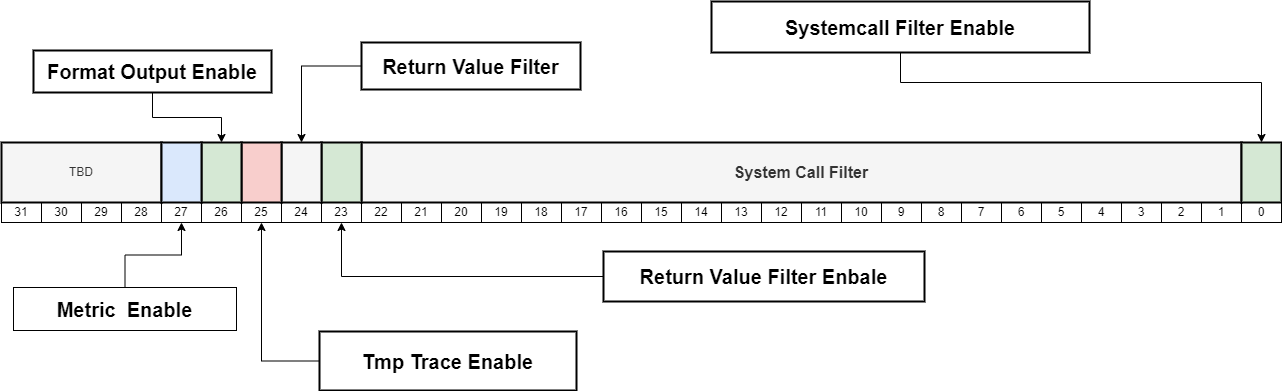
\includegraphics[width=4.75in]{pstrace.png}
    \centering
    \caption{"pstrace" in "proc"}
\end{figure}


\begin{quotation}
    Option -e [system call name]:
    When option flag -e is provided followed by a system call name, we will print only that
    system call. If no such system call is made in the command, print nothing.

    Option -s:
    When option flag -s is provided, print only successful system call.

    Option -f:
    When option flag -f is provided, print only failed system call.

    Option -s:
    Options -c in strace will generate a statistic report of system call regarding the input command
    such as duration, total call, and failed call. Create a similar report table using option -c.

    Option -f:
    When option flag -f is provided, print more readable output.

\end{quotation}

We have 21 syscalls on xv6 and 5 different options, so we can store this information
in a 32-bit variable. As you can see in the figure, I use 21+1 bit for the "-e" option. 


\paragraph*{Option -e}
The 0th bit is the inuse-bit of 1-22 bits. For example, if we don't run strace with
the "-e" flag the 0th bit is 0, the strace-kernel would not check the syscall filter.

\begin{figure}[H]
    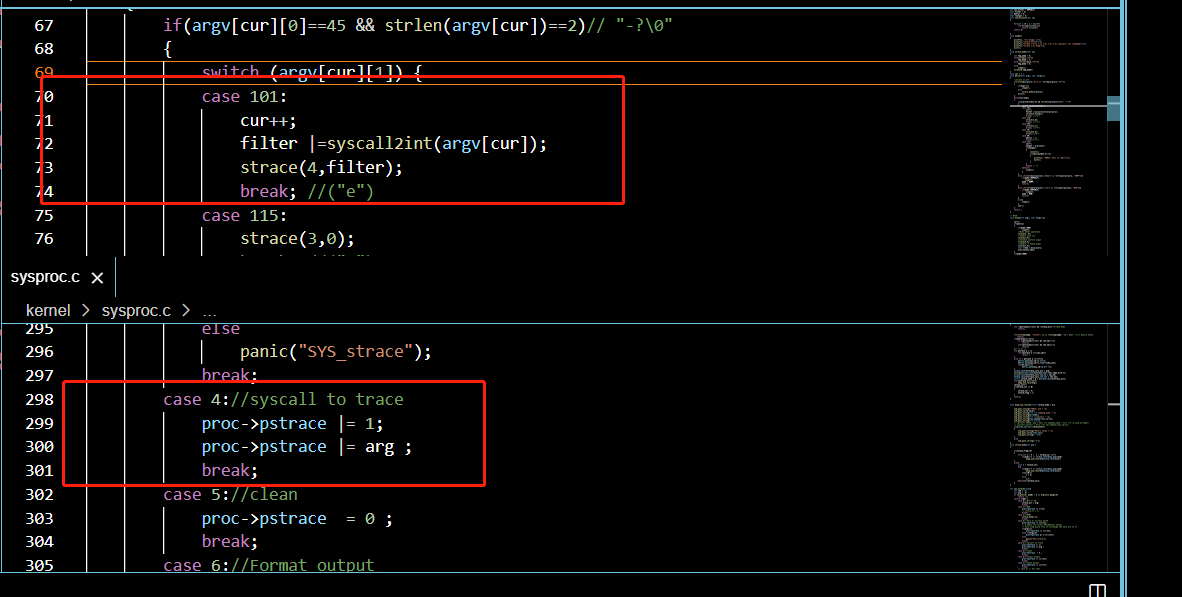
\includegraphics[width=4.75in]{1-20.png}
    \centering
    \caption{-e Opetion Implementation}
\end{figure}

The above figure is the user space and the kernel space handler of the "-e" operation.
The userspace handler would use a strace syscall to pass the filter to the kernel space 
which is a whitelist of syscalls while the kernel space would enable the syscall filter 
and apply the filter. 

\begin{figure}[H]
    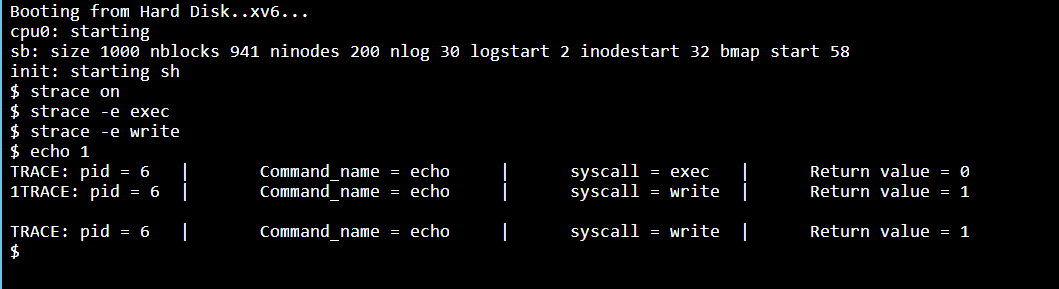
\includegraphics[width=4.75in]{1-21.png}
    \centering
    \caption{-e Opetion Demo}
\end{figure}


The above figure is a screenshot of the usage of the "-e" option and as you can see, 
my implementation could naturally handle the combination of the "-e" option.

\paragraph*{Option -s/f}

The 23rd and 24th bits of pstrace are designed for the "-s/f" flag. The 23rd bit is the 
inuse-bit of the 24th bit. And if the 24th bit is 0, the kernel would only record successful
syscalls while if the 24th bit is 1, the kernel would only record failed syscalls.

\begin{figure}[H]
    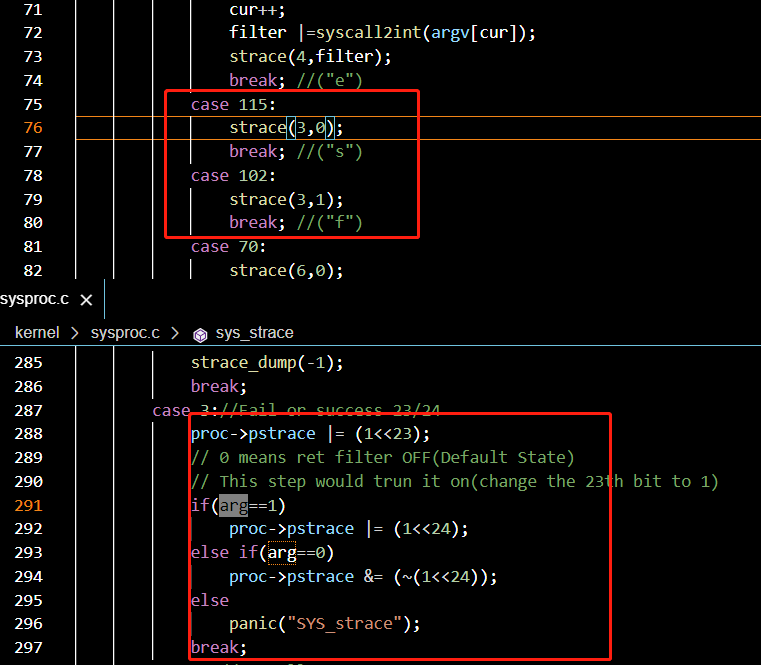
\includegraphics[width=4.75in]{1-22.png}
    \centering
    \caption{-s/f Opetion Implementation(Handler)}
\end{figure}

The above figure is the user space and the kernel space handler of the "-s/f" operation.
The user part would simply parse the arguments and call the kernel to apply the filter.
Also, the kernel-mode would apply the operation to the pstrace of the proc. And as you
can see in the beneath figure we will check the filter before printing out the syscall in "add\_one\_record".

\begin{figure}[H]
    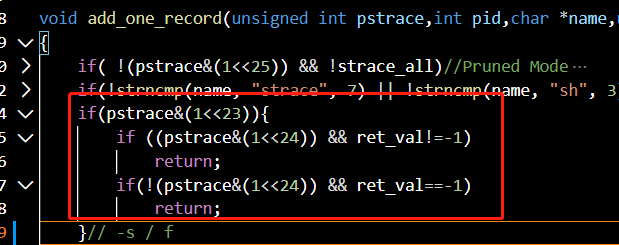
\includegraphics[width=4.75in]{1-23.png}
    \centering
    \caption{-s/f Opetion Implementation(Filter)}
\end{figure}

\begin{figure}[H]
    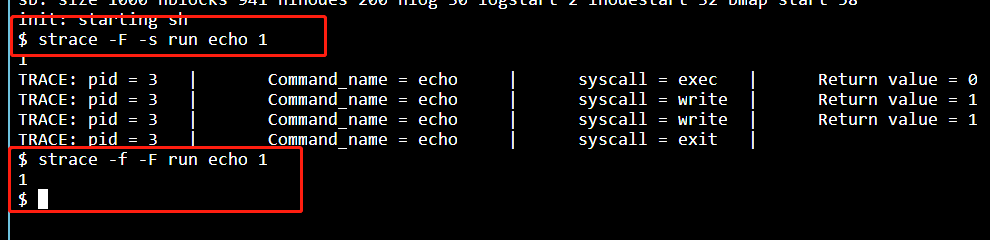
\includegraphics[width=4.75in]{1-26.png}
    \centering
    \caption{-s/f Opetion Demo}
\end{figure}

So far we finish the introduction of filter options (-s/f/e), and we'll move to format 
options in the following paragraphs.

\paragraph*{Option -F}
\begin{quotation}
    "Depends on your implementation, you might notice your command result is printed along with your
strace result which causes tracing to be difficult to read when characters keep mixing up between lines
(ex: 'ls' has a very long list result). Choose one of the following approaches to solve this issue:"
\end{quotation}

\begin{figure}[H]
    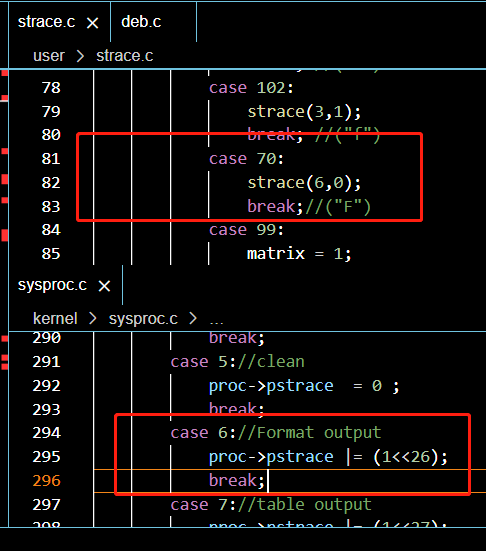
\includegraphics[width=4.75in]{1-27.png}
    \centering
    \caption{-F Opetion Implementation(Handler)}
\end{figure}

For this option, we need to "pause" the state output until the process finished its output.
So I would store the output in someplace and dump it after the process exits by reusing partial 
code of the "DUMP" sub-command. This is quite simple and elegant but it has a little flaw: What if
the process class tons of syscall and we could only store the latest N records. 

\begin{figure}[H]
    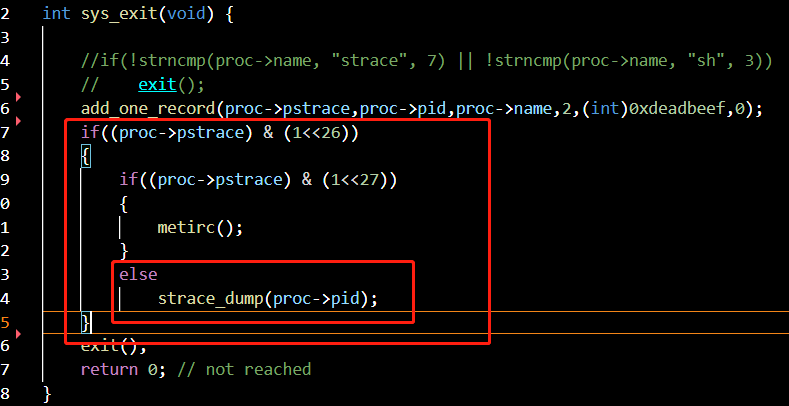
\includegraphics[width=4.75in]{1-24.png}
    \centering
    \caption{-F Opetion Implementation}
\end{figure}

For this issue, I can just set a variable to monitor the storage and dump the records if 
we are in "-F" mode. But I think this method would break XV6's simply so I would rather 
mention this issue in the README.md. And the following figure shows the output of the "-F" option.

\begin{figure}[H]
    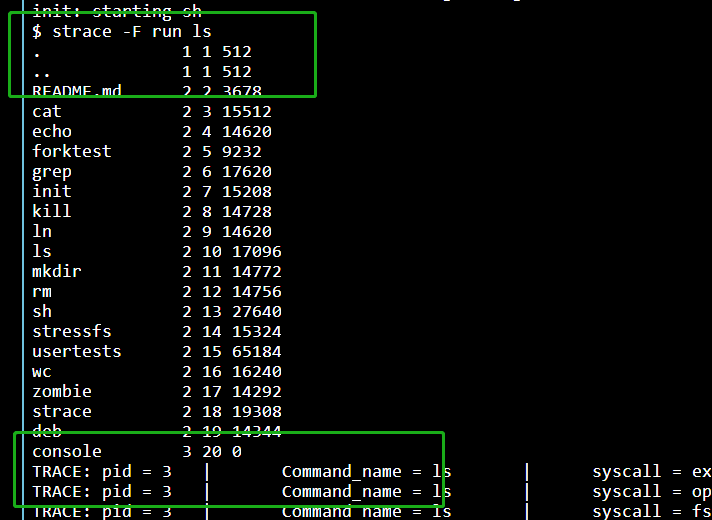
\includegraphics[width=4.75in]{1-25.png}
    \centering
    \caption{-F Opetion Demo}
\end{figure}

\paragraph*{Option -c}
\begin{quotation}
    "Options -c in strace will generate a statistic report of system call regarding the input command
    such as duration, total call, failed call. Create a similar report table using option -c."
\end{quotation}

\begin{figure}[H]
    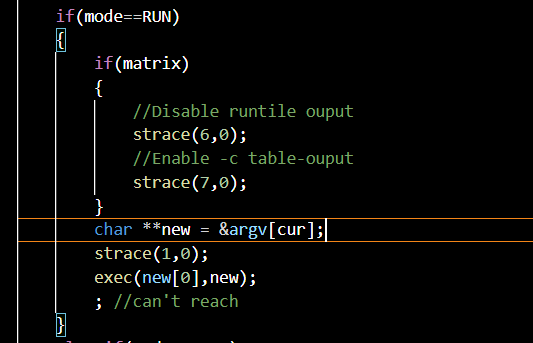
\includegraphics[width=4.75in]{1-37.png}
    \centering
    \caption{-C Option User Space Implementation}
\end{figure}

The "-c" would show the metrics of the command. We need to store more information about 
the syscalls so that allocating more space is necessary. 
For time recording, I would use uptime syscall to calculate the time used for every syscall.
And it's easy to count the error number and usage number in function "add\_one\_record".
\begin{figure}[H]
    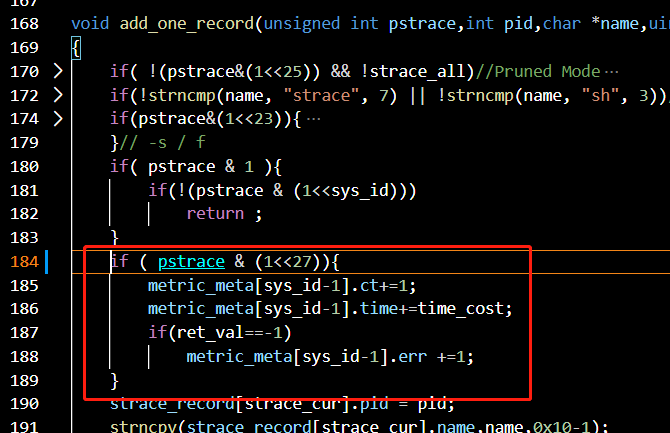
\includegraphics[width=4.75in]{1-30.png}
    \centering
    \caption{-C Option Implementation}
\end{figure}
And just before the exit, the "metric" function would be triggered and dump the "-c" 
related informations as the following figure.
\begin{figure}[H]
    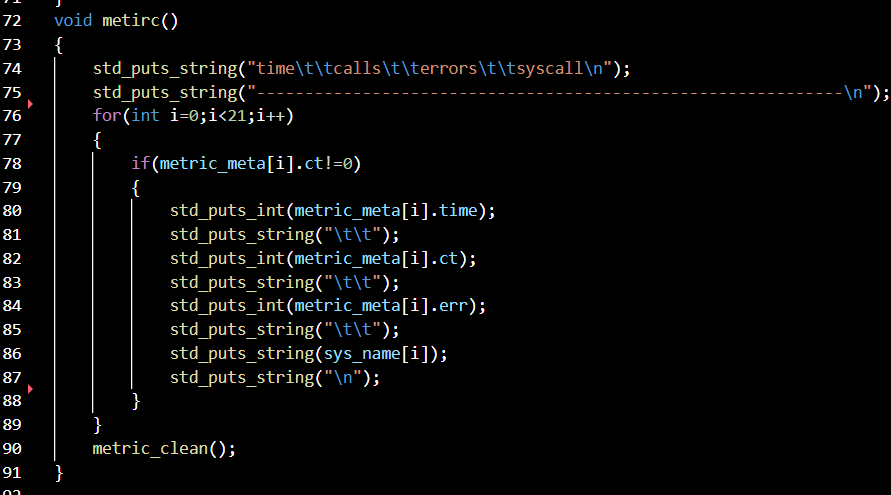
\includegraphics[width=4.75in]{1-31.png}
    \centering
    \caption{-c Option Demo}
    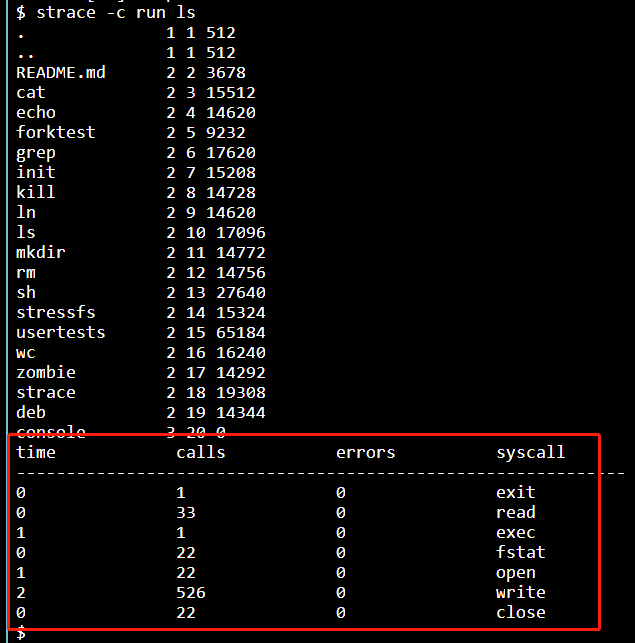
\includegraphics[width=4.75in]{1-32.png}
    \centering
    \caption{-c Option Demo}
\end{figure}
And it's great to know "even" costs such much (33 times more than reading)!

\paragraph*{Option -o}
\begin{quotation}
    "Find an implementation of choice to write strace output to file.
    For example: by providing option: -o 'filename' or editing content of README."
\end{quotation}

\begin{figure}[H]
    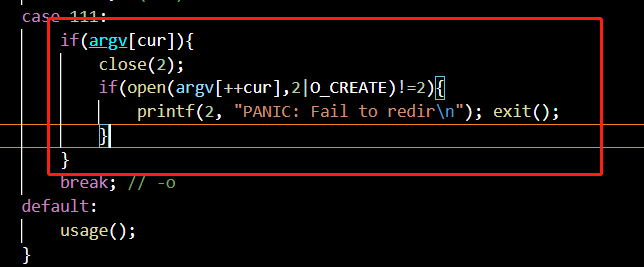
\includegraphics[width=4.75in]{1-33.png}
    \centering
    \caption{-o Option Userspace Handler}
\end{figure}

This one is the hardest one for my implementation because I use "exec" to run the command
rather than the fork. So I need to handle all the things in the kernel which is not secure.
As you see in the above figure, I can easily finish the userspace interface. Similar to what 
we learned in "sh.c", I just redirect the stderr to the given file. 

\begin{figure}[H]
    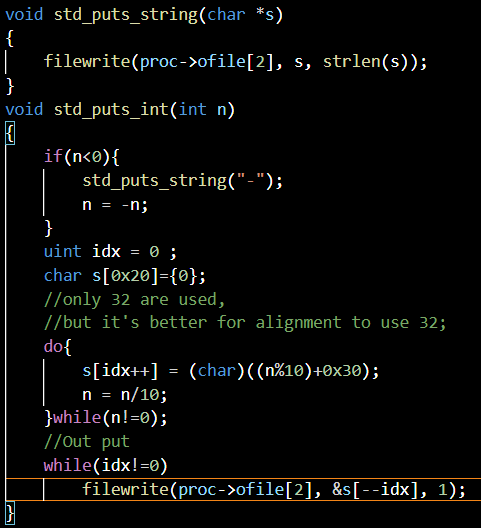
\includegraphics[width=4.75in]{1-34.png}
    \centering
    \caption{Format Print in Kernel}
\end{figure}

But unluckily, we don't have "printf" in the kernel to store the data into stderr.
So I need to implement a limited "printf" to store the output to the stdin out. 
I use the read file to achieve that as the above code shows. I replace all output functions
with my "format print" functions so that "-o" could naturally work with other 
commands and options, which is shown in the beneath figure.

\begin{figure}[H]
    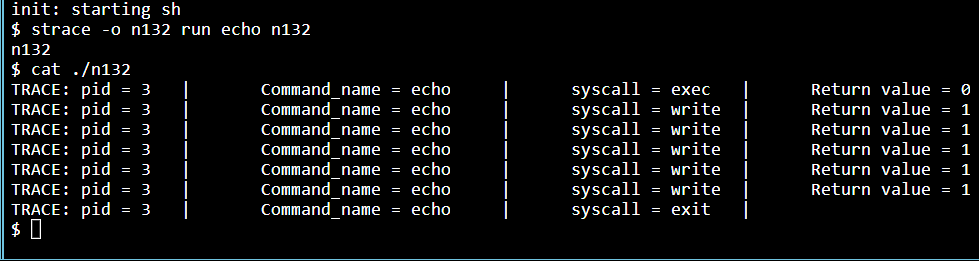
\includegraphics[width=4.75in]{1-35.png}
    \centering
    \caption{-o Opetion Demo}
\end{figure}

\section{Application to strace}

\begin{quotation}
    "Write a small program that produces an unexpected behavior such as race condition, delay output, crash
    on condition, memory leak, or your choice of implementation. Run strace on this program."
\end{quotation}

\begin{figure}[H]
    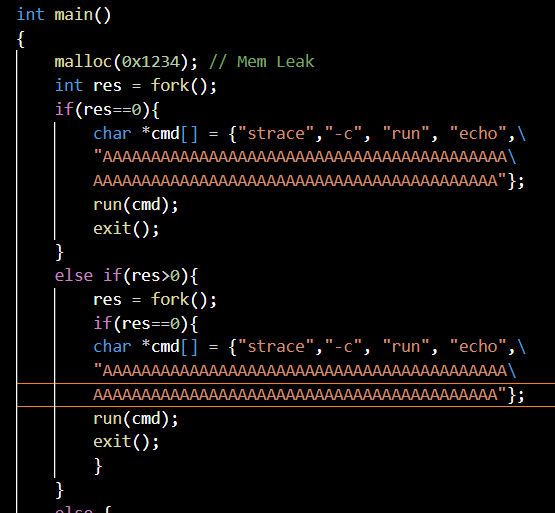
\includegraphics[width=4.75in]{1-40.png}
    \centering
    \caption{Race Condition TestCase}
\end{figure}

I wrote a simple test case.c to see if there are some race condition problems without the "-c" option. And we 
could clearly see the demo results in race conditions. It's unexcepted. The except result should be 
two same tables for each subprocess. I'll fix it in this section.

I used to store the "-c" option-related data in a global variable. And if there are two processes using it,
the output may be hard to accept because the first exited process would clean the variable. 

\begin{figure}[H]
    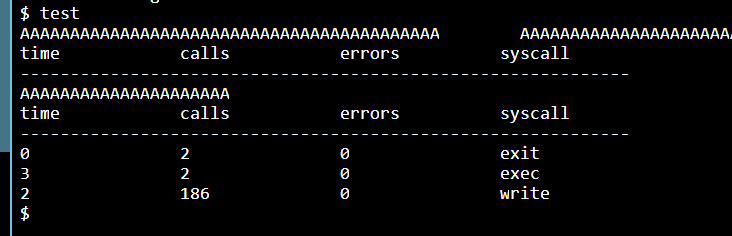
\includegraphics[width=4.75in]{1-41.png}
    \centering
    \caption{Race Condition Found}
\end{figure}

\paragraph*{How to Fix} 
We could let the process possess the struct so different processes would have different variables to store 
their syscall records. So I change the global variable to a process-owned variable and disable the interrupts
while dumping the output. 

\begin{figure}[H]
    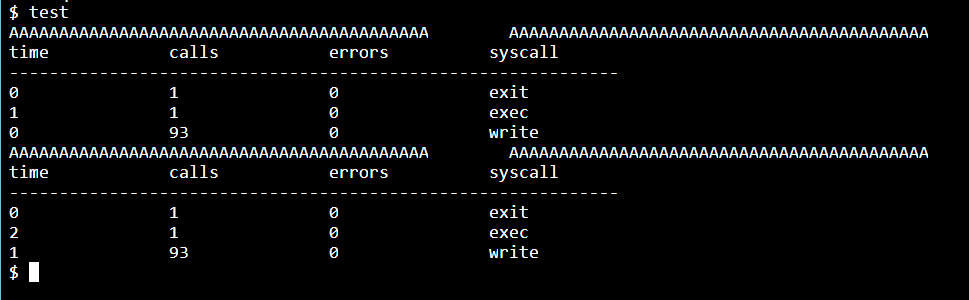
\includegraphics[width=4.75in]{1-42.png}
    \centering
    \caption{Race Condition Fixed}
\end{figure}

As you can see in the above figure, the output keeps the correct order and the number of syscalls is correct!

\begin{figure}[H]
    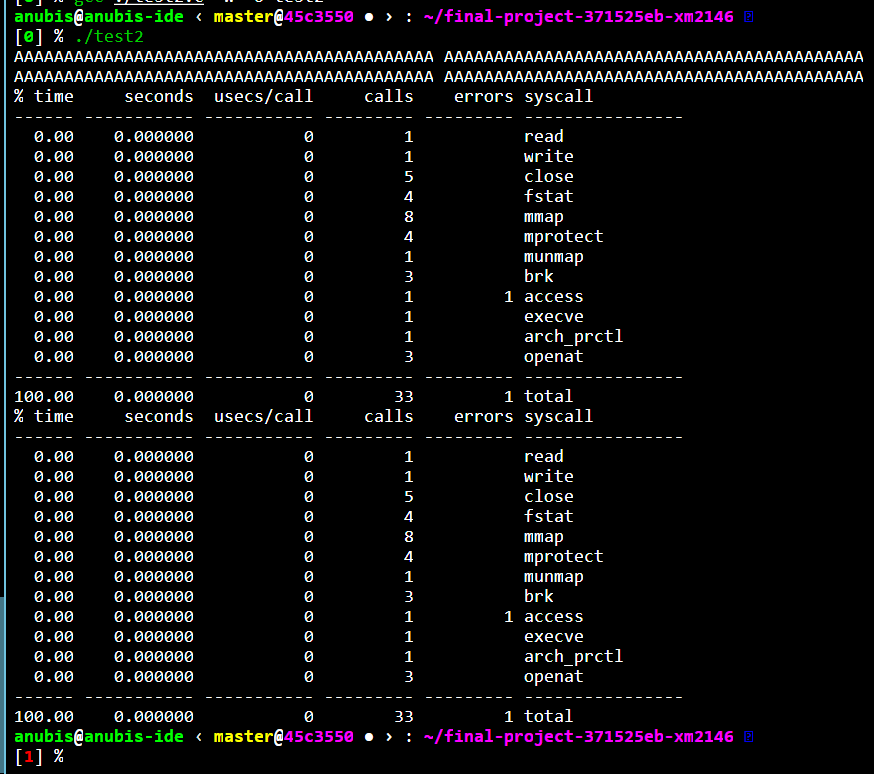
\includegraphics[width=4.75in]{1-43.png}
    \centering
    \caption{Same Program on Linux}
\end{figure}

Besides, I implemented a functionally same program in test2.c. The Linux starts surely provides one 
thing than our process, the time ratio. It could show the ratio of time cost by different syscalls.
And both strace can't help me find the data leak because it's a dynamic issue and the strace would not
trace all the allocated memory in the process.

\begin{figure}[H]
    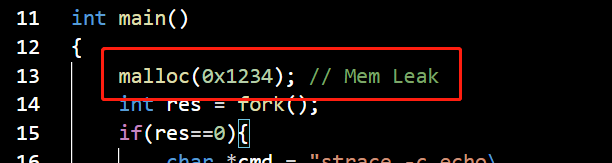
\includegraphics[width=4.75in]{1-44.png}
    \centering
    \caption{Memory Leak}
\end{figure}

\paragraph*{More Testing}
Also, I write lots of test cases to test my strace in /Test\_Log.MD.

\section{Todo}

During the implementation and the testing, I noticed there are several flaws in my 
implementation. And I decide to leave these flaws in my code 
because I didn't have time to improve these issues and this is an educational assignment
rather than a product.

\paragraph*{Strace RUN}
For strace run, it's better to use a fork because for some options we need to store the 
data until the process exits. So we need a parent process to wait for the child to process 
as a daemon and finish the output task after the child process exits, as it's more 
secure to write a file in userspace.

\paragraph*{-F Option}
This is a special issue with the -F option which aims at printing more readable output.
To protect the simplicity of the xv6 kernel, I decide not to implement a mechanism
to deal with infinity syscall records. So if there are more than N records when running
the command, I would only print out the last N records rather than all the records.

\paragraph*{Race Condition}
We should be very paranoid about the kernel global variables. If there is more than one
process, we may have race conditions! I didn't think much about this and only did some
simple testing on that. More paranoid code reviews should be taken for any code in the kernel.


\section{Structure of Strace}

\begin{figure}[H]
    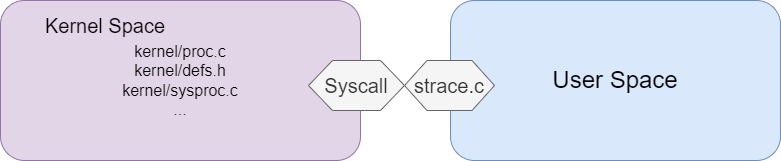
\includegraphics[width=4.75in]{1-36.png}
    \centering
    \caption{Structure}
\end{figure}
There are two main parts of this implementation: Kernel Space Part and User Space Part.

In the user space, I use the binary strace as the interface to
transfer data to the kernel. And the main handler is the file "kernel/proc.c". I
implement a strace syscall and deal with kinds of parameters. 

In the kernel space, I use the metadata got from the strace syscall to set the
output format/filter options. Also, I use the kernel variables to implement
"strace on/off". And you can check all the supported features in the above figure.


\begin{figure}[H]
    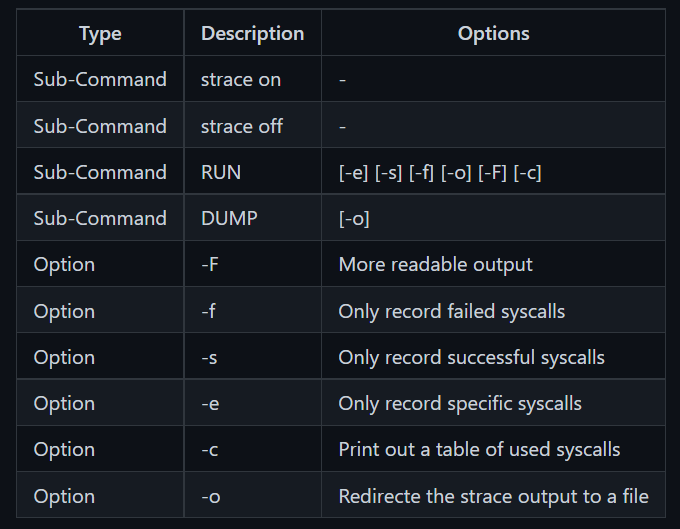
\includegraphics[width=4.75in]{1-39.png}
    \centering
    \caption{Supported Features}
\end{figure}


\section{Summary}

\begin{figure}[H]
    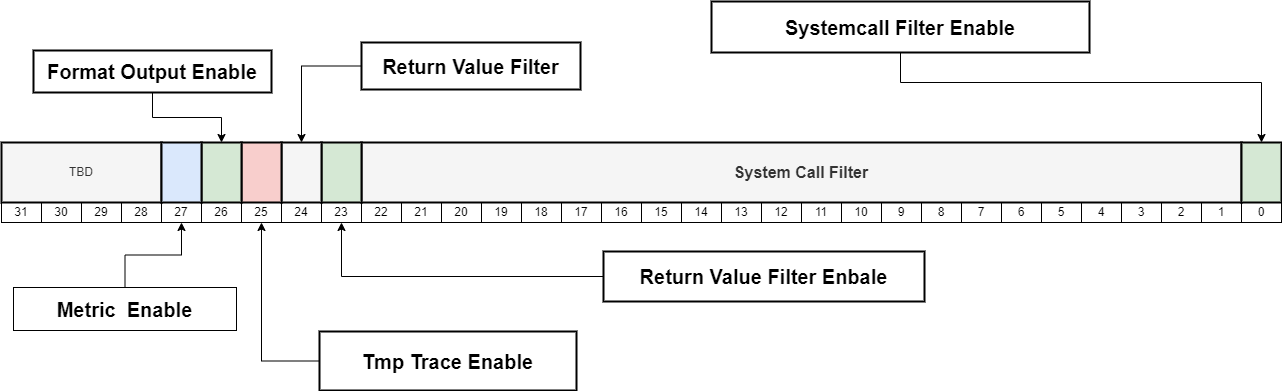
\includegraphics[width=4.75in]{pstrace.png}
    \centering
    \caption{My Strace}
\end{figure}

The above figure is my pstrace's structure I spent lots of time on it to make it elegant.
I am really happy I didn't waste the opportunity
to push myself. As a result, I learned a lot during this assignment and have a more 
complete view of the Unix kernel. And I could feel that the knowledge I learned on 
the course and the xv6 could be used to understand really Linux kernel. 

\end{document}